%                                                                 aa.dem
% AA vers. 8.2, LaTeX class for Astronomy & Astrophysics
% demonstration file
%                                                       (c) EDP Sciences
%-----------------------------------------------------------------------
%
%documentclass[referee]{aa} % for a referee version
%\documentclass[onecolumn]{aa} % for a paper on 1 column  
%\documentclass[longauth]{aa} % for the long lists of affiliations 
%\documentclass[rnote]{aa} % for the research notes
%\documentclass[letter]{aa} % for the letters 
%\documentclass[bibyear]{aa} % if the references are not structured 
% according to the author-year natbib style

%
\documentclass{aa}  

%
\usepackage{graphicx}
%%%%%%%%%%%%%%%%%%%%%%%%%%%%%%%%%%%%%%%%
\usepackage{txfonts}
%%%%%%%%%%%%%%%%%%%%%%%%%%%%%%%%%%%%%%%%
%\usepackage[options]{hyperref}
% To add links in your PDF file, use the package "hyperref"
% with options according to your LaTeX or PDFLaTeX drivers.
%
\begin{document} 


   \title{Subarray optimization in radio interferometry using a Genetic Algorithm}

   \subtitle{ALMA case}

   \author{S. Leon\inst{1}, R. Lassis
          \inst{2}
          \and
          B. Vila-Vilaro\inst{1}
          }

   \institute{Joint ALMA Observatory, European Southern Observatory, \\
              Santiago, Chile \\
              \email{stephane.leon@alma.cl}
         \and
             INSA, Toulouse, France\\
             \email{roxanelassis@gmail.com}
             }

   \date{Received xx; accepted xx}

% \abstract{}{}{}{}{} 
% 5 {} token are mandatory
 
  \abstract
  % context heading (optional)https://www.sharelatex.com/project/5aa7e4def3674a4ba4d505d8
  % {} leave it empty if necessary  
  {zzzzz}
  % aims heading (mandatory)
   {It is shown that stability
   depends only upon the equations of state, the opacities and the local
   thermodynamic state in the layer. Stability and instability can
   therefore be expressed in the form of stability equations of state
   which are universal for a given composition.}
  % methods heading (mandatory)
   {zzzzz}
  % results
   {zzzzzz}
  % conclusions heading (optional), leave it empty if necessary 
   {zzzzzzzzzzzzzzzzz}

   \keywords{radio astronomy -- interferometry technique
               }

   \maketitle
%
%-------------------------------------------------------------------

\section{Introduction}

In astronomy the technique of synthesis aperture is taking advantage of the Van Cittert-Zernike theorem to fill the Fourier plane of the sky emission  by
performing interferometric observations. For several decades the observations in the radio domain were done by interferometry  by correlating the signal from 
receivers installed in the focal plane of antennas located at different positions. The first observations by interferometry were performed in radio because of the 
large wavelengths compared to others astronomical windows which allow an easier controlled delay correction. Historically the first radio interferometers were build for 
low frequency observations like XXX  operating at XXX GHz. 

A long standing problem and debate  in radio interferometry is the locations of the antennas forming the array (see XXX,XXX,XXX). The natural earth rotation is combined to the
baseline vectors formed by the antenna pairs to measure the sky intensity in the Fourier plane. Depending on the number of antennas, i.e. the number of baselines, the quality
of the image depends strongly on the antenna location. The correlated signal of an antenna pair is called a visibility V(l,m) in radio astronomy. According to the type of
receiver these visibilities can be obtained either at different frequencies for a spectral data cube in the Fourier plane or formed on a large bandwidth for a continuum dataset.

Different strategies have been employed to optimize the  array configurations like for the XXX, XXX, XXX and XXXX. Image quality, spatial resolution, sensitivity and 
antenna logistic, like the number of antennas and  the possibility of relocation, are the main drivers for the optimization of an array configuration. 

The Section \ref{secAC} exposes the array and subarray configuration, Section \ref{secGA} presents the Genetic Algorithm for optimization and Section \ref{secRes} and \ref{secDiscussion} presents and discuss the results of the subarray selection algorithm for the ALMA case.


%--------------------------------------------------------------------
\section{Array Configuration}
\label{secAC}

The instantaneous location of the $N_a$ antenna of an array defines its properties to recover the spatial emission of the astronomical object. Following
the ALMA Technical Handbook (XXX) nomenclature we can define the visibilities $\mathcal{V}$(u,v) in the uv-plane as the Fourier Transform of the sky emission.
In the rest of the article we only consider the 2D distribution of the visibilities assuming a coplanar distribution.

\subsection{Description}

The relationship between the sky brightness distribution $I(l,m)$ and the complex visibility distribution $\mathcal{V}(u,v)$ is described by the Van Cittert-Zernike theorem as follows : 
	
	\begin{equation}
	\mathcal{V}(u,v) =\int \int I(l,m)e^{2\pi i(ul+vm)}dldm
	\end{equation}
	
Nonetheless, this expression is true for idealized antennas. Each antenna of the radio interferometer has a finite diameter and then its own power response 
$\mathcal{A}(l,m)$ for its coupling with the sky emission. The correlator output is then:
	
	\begin{equation}
	\mathcal{V}(u,v) =\int \int \mathcal{A}(l,m)I(l,m)e^{2\pi i(ul+vm)}dldm
	\end{equation}
	
where $\mathcal{A}(l,m)$ is the antenna response function.
	
To recover the sky emission image it is necessary to perform a deconvolution process on the visibilities. Several algorithms have been developed  for that operation. In radio astronomy several deconvolution algorithms are derived from the "Clean" algorithm described for the first time by Hogbom et al. (1975). The main idea for the algorithm is to Fourier transform the sampled visibilities into the so-called dirty image and iteratively extract the signal as a Dirac set of emission. The final image is restored by summing the Dirac detection convolved by the fitted Gaussian beam on the sampling of the visibilities in the Fourier domain.
That Gaussian beam gives directly the spatial resolution of the final image, it is defined by respectively the minor, major axis and position angle of the 2D Gaussian beam
Because of the sampling in the Fourier domain only some spatial scales are recovered, the smallest spatial scales
are given by the Gaussian beam and the largest spatial scales are estimated by the Maximum Recovered Scale (MRS) parameter. The MRS is computed hereafter by the angular scale of the minimum baseline length at the observation frequency.

	
\subsection{Subarray}

In some situation (calibration, science) it is necessary to divide the array in N subarrays devoted to different
tasks. Each subarray is defined by its own constraint such as number of antennas, spatial resolution, image quality, MRS.

%--------------------------------------------------------------------

\section{Genetic Algorithm}
\label{secGA}




\subsection{Description}

aaaaaaa
\subsection{Subarray selection}


\subsection{Metrics and implementation}

aaaaaaaaaaaaaa

%-----------------------------------------------------------------------
\section{Results}
\label{secRes}


aaaaaaa

%---------------------------------------------------------------------

\section{Discussion}
\label{secDiscussion}

AAAAAAAAAAAAAAAAAAaa


%-----------------------------------------------------------------

\section{Conclusions}

   \begin{enumerate}
      \item first conclusion
   \end{enumerate}

\begin{acknowledgements}
      Part of this work was supported by the German
      \emph{Deut\-sche For\-schungs\-ge\-mein\-schaft, DFG\/} project
      number Ts~17/2--1.
\end{acknowledgements}

% WARNING
%-------------------------------------------------------------------
% Please note that we have included the references to the file aa.dem in
% order to compile it, but we ask you to:
%
% - use BibTeX with the regular commands:
%   \bibliographystyle{aa} % style aa.bst
%   \bibliography{Yourfile} % your references Yourfile.bib
%
% - join the .bib files when you upload your source files
%-------------------------------------------------------------------

\begin{thebibliography}{}

  \bibitem[Baker(1966)]{baker} Baker, N. 1966,
      in Stellar Evolution,
      ed.\ R. F. Stein,\& A. G. W. Cameron
      (Plenum, New York) 333

   \bibitem[Balluch(1988)]{balluch} Balluch, M. 1988,
      A\&A, 200, 58

   \bibitem[Cox(1980)]{cox} Cox, J. P. 1980,
      Theory of Stellar Pulsation
      (Princeton University Press, Princeton) 165

   \bibitem[Cox(1969)]{cox69} Cox, A. N.,\& Stewart, J. N. 1969,
      Academia Nauk, Scientific Information 15, 1

   \bibitem[Mizuno(1980)]{mizuno} Mizuno H. 1980,
      Prog. Theor. Phys., 64, 544
   
   \bibitem[Tscharnuter(1987)]{tscharnuter} Tscharnuter W. M. 1987,
      A\&A, 188, 55
  
   \bibitem[Terlevich(1992)]{terlevich} Terlevich, R. 1992, in ASP Conf. Ser. 31, 
      Relationships between Active Galactic Nuclei and Starburst Galaxies, 
      ed. A. V. Filippenko, 13

   \bibitem[Yorke(1980a)]{yorke80a} Yorke, H. W. 1980a,
      A\&A, 86, 286

   \bibitem[Zheng(1997)]{zheng} Zheng, W., Davidsen, A. F., Tytler, D. \& Kriss, G. A.
      1997, preprint
\end{thebibliography}


%%%%%%%%%%%%%%%%%%%%%%%%%%%%%%%%%%%%%%%%%%%%%%%%%%%%%%%%%%%%%%%%%%%%%%%%%%%%%%%%%%%%%%%%%%%%%%%%%
%%%%%%%%%%%%%%% critical antenna algorithm

\begin{appendix}

\section{Visibilities and critical antenas}

A snapshot observation by a given array can be described by a list of n antennas(= pads) $a_i$ (i = 1 .. n). Each pair of antenna $(a_i,a_j)$ produce a visibility $V_{ij}$ 
at the location $\overrightarrow{a_ia_j}$ in the uv-plan (snapshot mode).

\subsection{Voronoi tessalation in the uv-plan}

We perform the Voronoi tessalation of the visibilities $V_{ij}$ in the UV-plan as shown on the Fig.  \ref{fig_vor}. Each visibility $V_{ij}$ is associated with 
the corresponding Voronoi area $S_{ij}$.


\begin{figure*}
 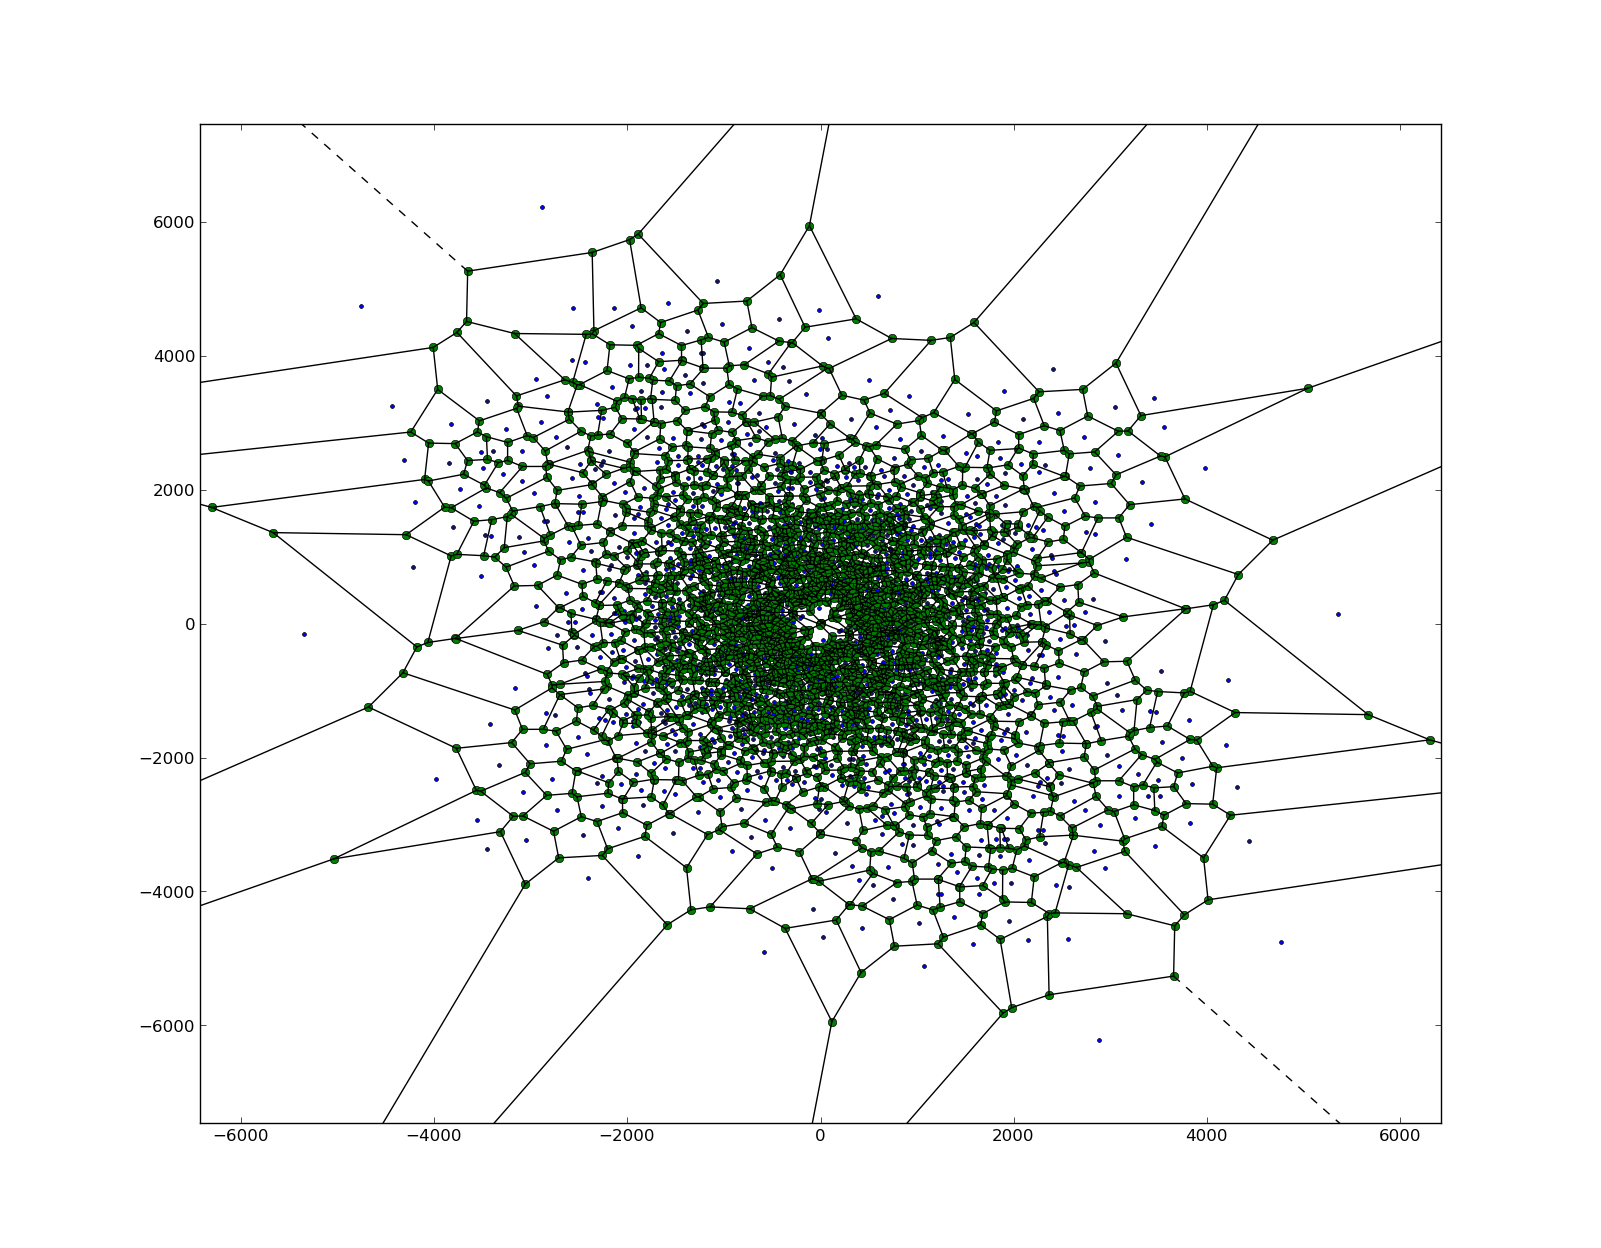
\includegraphics[width=15cm]{O-21-voronoi.png}
 \caption{Voronoi tesselation of the visibilities $V_{ij}$ in the uv-plan for a snapshot observation. Each point is a visibility $V_{ij}$ which can be associated
 with the Voronoi area $S_{ij}$. That example corresponds to the standard configuration O-21 for the ALMA 12-m array with 50 antennas.}
 \label{fig_vor}
\end{figure*}





\subsection{Normalised antenna criticality parameter}


The criticality of  a given antenna i for an observation can be estimated by the sum of all the area $S_{ij}$ associated with that antenna. It is equivalent to 
the total area covered by the visibilities related to an antenna in the uv-plan. We assume that all antennas are used to produce the final image. We call it the
criticality $C_i$ :

\begin{equation}
 C_i = \sum_{k = 1}^{n} \alpha _{ik} S_{ik}
\end{equation}

where $S_{ij}$ is the Voronoi area of the visibility $V_{ij}$, $\alpha_{ij}$ is a weight applied, if necessary, on the pair of antennas i and j. According to that criteria the most critical antenna $a_M$  would be the one with the largest criticality parameter $C_i$ :

\begin{equation}
 C_M = max(C_i)
\end{equation}

We can normalize the criticality parameters with respect to the most critical antenna by defining the  normalised criticality parameters $C_i^n$ as following :

\begin{equation}
    C_i^n = \frac{C_i}{C_M}
    \label{eqn_normvoronoi}
\end{equation}


Finally we can sort the (normalised) criticality parameters to give the list of the critical antennas from the most critical $a_M$ to the least critical $a_m$ with:

\begin{equation}
    C_M^n = 1 > ... C_i^n > ... > C_m^n
\end{equation}

The normalisation of the criticality parameter can be understood as a relative contribution of the area of all the visibilities contributed by an antenna wrt. to the most critical antenna.

If the system temperature $T_i$ is available for each antenna i, the following weighting $\alpha_{ij}$ can be applied :
\begin{equation}
\alpha_{ij} = \frac{1}{T_iT_j}    
\end{equation}



\subsection{Example for an ALMA configuration}

We select the ALMA array configuration of the 12-m array located at 5000m altitude the 28/11/2016 (see Fig. \ref{fig_pospads}). There are 49 antennas distributed 
on the pads with a maximum baseline of 704 m and a minimum baseline of 15 m. The spatial resolution with a Brigg  parameter R = 0.5 is 0.9673 arcsec at a frequency of 
100 GHz. 


\begin{figure*}
 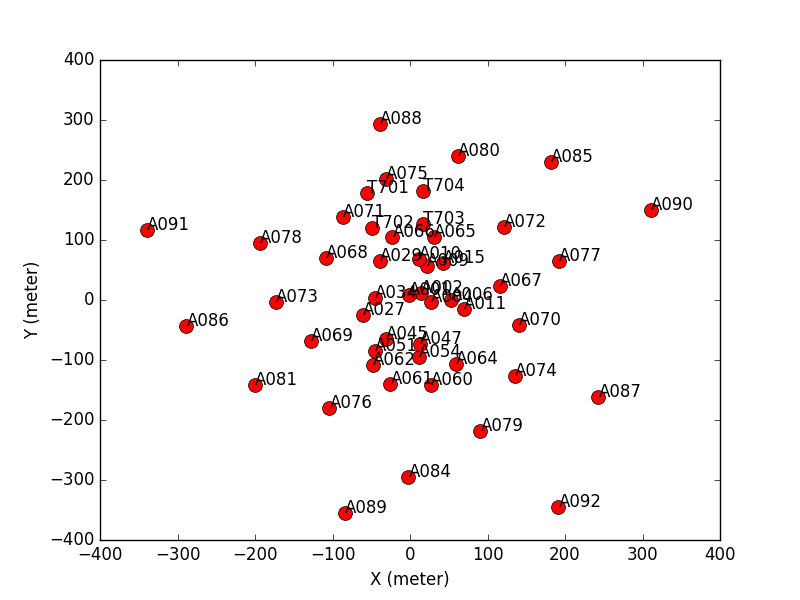
\includegraphics[width=15cm]{posPads.png}
 \caption{Position of the pads for the ALMA 12-m configuration the 28/11/2016.}
 \label{fig_pospads}
\end{figure*}

Using the normalized criticality parameter defined in \ref{eqn_normvoronoi} and a uniform weighting ($\alpha_{ij} = 1$)  we obtain the list of the critical antenna pads starting with the most
critical antenna (100 \%):

\begin{verbatim}
    A090 [100.00 %]  A081 [80.03 %]  A092 [71.92 %]  A091 [54.10 %]  A089 [43.37 %]  
    A086 [42.62 %]  A080 [39.47 %]  A087 [35.74 %]  A085 [35.39 %]  A084 [34.26 %]  
    A078 [33.44 %]  A088 [25.33 %]  A077 [22.05 %]  A079 [20.96 %]  A073 [18.60 %]  
    A076 [18.04 %]  A075 [17.70 %]  T701 [16.87 %]  A072 [16.57 %]  A074 [15.44 %]  
    A071 [14.71 %]  T704 [13.53 %]  A069 [13.39 %]  A070 [12.03 %]  A067 [11.96 %]  
    A060 [11.46 %]  A068 [11.31 %]  A066 [9.56 %]  T703 [9.05 %]  T702 [9.01 %]  
    A061 [8.69 %]  A029 [8.61 %]  A062 [8.52 %]  A065 [8.37 %]  A064 [8.30 %]  
    A027 [8.21 %]  A045 [7.53 %]  A047 [7.33 %]  A015 [7.22 %]  A034 [7.06 %]  
    A001 [6.97 %]  A051 [6.90 %]  A054 [6.60 %]  A011 [6.49 %]  A009 [6.42 %]  
    A010 [6.36 %]  A006 [6.17 %]  A002 [5.94 %]  A004 [5.88 %]  

\end{verbatim}


The percentage in that  list can be interpreted as following, the pad A090 contributes to an area in the uv-plan 1.25 times larger than the pad A081 and, for example, 11.5 times larger that the pad A061.



\end{appendix}


\end{document}

%%%%%%%%%%%%%%%%%%%%%%%%%%%%%%%%%%%%%%%%%%%%%%%%%%%%%%%%%%%%%%%%%%%%%%%%%%%%%%%%%%%%%%%%%%%%%%%%%%%%%%%%%%%%%%%%%%%%%%%%%%%%%%
%%%%%%%%%%%%%%%%%%%%%%%%%%%%%%%%%%%%%%%%%%%%%%%%%%%%%%%%%%%%%%%%%%%%%%%%%%%%%%%%%%%%%%%%%%%%%%%%%%%%%%%%%%%%%%%%%%%%%%%%%%%%%
%%%%%%%%%%%%%%%%%%%%%%%%%%%%%%%%%%%%%%%%%%%%%%%%%%%%%%%%%%%%%%%%%%%%%%%%%%%%%%%%%%%%%%%%%%%%%%%%%%%%%%%%%%%%%%%%%%%%%%%%%%%%%%
%%%%%%%%%%%%%%%%%%%%%%%%%%%%%%%%%%%%%%%%%%%%%%%%%%%%%%%%%%%%%%%%%%%%%%%%%%%%%%%%%%%%%%%%%%%%%%%%%%%%%%%%%%%%%%%%%%%%%%%%%%%%%%






%%%%%%%%%%%%%%%%%%%%%%%%%%%%%%%%%%%%%%%%%%%%%%%%%%%%%%%%%%%%%%
Example below of non-structurated natbib references  
To use the v8.3 macros with this form of composition of bibliography, 
the option "bibyear" should be added to the command line 
"\documentclass[bibyear]{aa}".
%%%%%%%%%%%%%%%%%%%%%%%%%%%%%%%%%%%%%%%%%%%%%%%%%%%%%%%%%%%%%%

\begin{thebibliography}{}

  \bibitem[1966]{baker} Baker, N. 1966,
      in Stellar Evolution,
      ed.\ R. F. Stein,\& A. G. W. Cameron
      (Plenum, New York) 333

   \bibitem[1988]{balluch} Balluch, M. 1988,
      A\&A, 200, 58

   \bibitem[1980]{cox} Cox, J. P. 1980,
      Theory of Stellar Pulsation
      (Princeton University Press, Princeton) 165

   \bibitem[1969]{cox69} Cox, A. N.,\& Stewart, J. N. 1969,
      Academia Nauk, Scientific Information 15, 1

   \bibitem[1980]{mizuno} Mizuno H. 1980,
      Prog. Theor. Phys., 64, 544
   
   \bibitem[1987]{tscharnuter} Tscharnuter W. M. 1987,
      A\&A, 188, 55
  
   \bibitem[1992]{terlevich} Terlevich, R. 1992, in ASP Conf. Ser. 31, 
      Relationships between Active Galactic Nuclei and Starburst Galaxies, 
      ed. A. V. Filippenko, 13

   \bibitem[1980a]{yorke80a} Yorke, H. W. 1980a,
      A\&A, 86, 286

   \bibitem[1997]{zheng} Zheng, W., Davidsen, A. F., Tytler, D. \& Kriss, G. A.
      1997, preprint
\end{thebibliography}
%
%%%%%%%%%%%%%%%%%%%%%%%%%%%%%%%%%%%%%%%%%%%%%%%%%%%%%%%%%%%%%%
Examples for figures using graphicx
A guide "Using Imported Graphics in LaTeX2e"  (Keith Reckdahl)
is available on a lot of LaTeX public servers or ctan mirrors.
The file is : epslatex.pdf 
%%%%%%%%%%%%%%%%%%%%%%%%%%%%%%%%%%%%%%%%%%%%%%%%%%%%%%%%%%%%%%

%-------------------------------------------------------------
%                 A figure as large as the width of the column
%-------------------------------------------------------------
   \begin{figure}
   \centering
   \includegraphics[width=\hsize]{empty.eps}
      \caption{Vibrational stability equation of state
               $S_{\mathrm{vib}}(\lg e, \lg \rho)$.
               $>0$ means vibrational stability.
              }
         \label{FigVibStab}
   \end{figure}
%
%-------------------------------------------------------------
%                                    One column rotated figure
%-------------------------------------------------------------
   \begin{figure}
   \centering
   \includegraphics[angle=-90,width=3cm]{empty.eps}
      \caption{Vibrational stability equation of state
               $S_{\mathrm{vib}}(\lg e, \lg \rho)$.
               $>0$ means vibrational stability.
              }
         \label{FigVibStab}
   \end{figure}
%
%-------------------------------------------------------------
%                        Figure with caption on the right side 
%-------------------------------------------------------------
   \begin{figure}
   \sidecaption
   \includegraphics[width=3cm]{empty.eps}
      \caption{Vibrational stability equation of state
               $S_{\mathrm{vib}}(\lg e, \lg \rho)$.
               $>0$ means vibrational stability.
              }
         \label{FigVibStab}
   \end{figure}
%
%-------------------------------------------------------------
%                                Figure with a new BoundingBox 
%-------------------------------------------------------------
   \begin{figure}
   \centering
   \includegraphics[bb=10 20 100 300,width=3cm,clip]{empty.eps}
      \caption{Vibrational stability equation of state
               $S_{\mathrm{vib}}(\lg e, \lg \rho)$.
               $>0$ means vibrational stability.
              }
         \label{FigVibStab}
   \end{figure}
%
%-------------------------------------------------------------
%                                      The "resizebox" command 
%-------------------------------------------------------------
   \begin{figure}
   \resizebox{\hsize}{!}
            {\includegraphics[bb=10 20 100 300,clip]{empty.eps}
      \caption{Vibrational stability equation of state
               $S_{\mathrm{vib}}(\lg e, \lg \rho)$.
               $>0$ means vibrational stability.
              }
         \label{FigVibStab}
   \end{figure}
%
%-------------------------------------------------------------
%                                             Two column Figure 
%-------------------------------------------------------------
   \begin{figure*}
   \resizebox{\hsize}{!}
            {\includegraphics[bb=10 20 100 300,clip]{empty.eps}
      \caption{Vibrational stability equation of state
               $S_{\mathrm{vib}}(\lg e, \lg \rho)$.
               $>0$ means vibrational stability.
              }
         \label{FigVibStab}
   \end{figure*}
%
%-------------------------------------------------------------
%                                             Simple A&A Table
%-------------------------------------------------------------
%
\begin{table}
\caption{Nonlinear Model Results}             % title of Table
\label{table:1}      % is used to refer this table in the text
\centering                          % used for centering table
\begin{tabular}{c c c c}        % centered columns (4 columns)
\hline\hline                 % inserts double horizontal lines
HJD & $E$ & Method\#2 & Method\#3 \\    % table heading 
\hline                        % inserts single horizontal line
   1 & 50 & $-837$ & 970 \\      % inserting body of the table
   2 & 47 & 877    & 230 \\
   3 & 31 & 25     & 415 \\
   4 & 35 & 144    & 2356 \\
   5 & 45 & 300    & 556 \\ 
\hline                                   %inserts single line
\end{tabular}
\end{table}
%
%-------------------------------------------------------------
%                                             Two column Table 
%-------------------------------------------------------------
%
\begin{table*}
\caption{Nonlinear Model Results}             
\label{table:1}      
\centering          
\begin{tabular}{c c c c l l l }     % 7 columns 
\hline\hline       
                      % To combine 4 columns into a single one 
HJD & $E$ & Method\#2 & \multicolumn{4}{c}{Method\#3}\\ 
\hline                    
   1 & 50 & $-837$ & 970 & 65 & 67 & 78\\  
   2 & 47 & 877    & 230 & 567& 55 & 78\\
   3 & 31 & 25     & 415 & 567& 55 & 78\\
   4 & 35 & 144    & 2356& 567& 55 & 78 \\
   5 & 45 & 300    & 556 & 567& 55 & 78\\
\hline                  
\end{tabular}
\end{table*}
%
%-------------------------------------------------------------
%                                          Table with notes 
%-------------------------------------------------------------
%
% A single note
\begin{table}
\caption{\label{t7}Spectral types and photometry for stars in the
  region.}
\centering
\begin{tabular}{lccc}
\hline\hline
Star&Spectral type&RA(J2000)&Dec(J2000)\\
\hline
69           &B1\,V     &09 15 54.046 & $-$50 00 26.67\\
49           &B0.7\,V   &*09 15 54.570& $-$50 00 03.90\\
LS~1267~(86) &O8\,V     &09 15 52.787&11.07\\
24.6         &7.58      &1.37 &0.20\\
\hline
LS~1262      &B0\,V     &09 15 05.17&11.17\\
MO 2-119     &B0.5\,V   &09 15 33.7 &11.74\\
LS~1269      &O8.5\,V   &09 15 56.60&10.85\\
\hline
\end{tabular}
\tablefoot{The top panel shows likely members of Pismis~11. The second
panel contains likely members of Alicante~5. The bottom panel
displays stars outside the clusters.}
\end{table}
%
% More notes
%
\begin{table}
\caption{\label{t7}Spectral types and photometry for stars in the
  region.}
\centering
\begin{tabular}{lccc}
\hline\hline
Star&Spectral type&RA(J2000)&Dec(J2000)\\
\hline
69           &B1\,V     &09 15 54.046 & $-$50 00 26.67\\
49           &B0.7\,V   &*09 15 54.570& $-$50 00 03.90\\
LS~1267~(86) &O8\,V     &09 15 52.787&11.07\tablefootmark{a}\\
24.6         &7.58\tablefootmark{1}&1.37\tablefootmark{a}   &0.20\tablefootmark{a}\\
\hline
LS~1262      &B0\,V     &09 15 05.17&11.17\tablefootmark{b}\\
MO 2-119     &B0.5\,V   &09 15 33.7 &11.74\tablefootmark{c}\\
LS~1269      &O8.5\,V   &09 15 56.60&10.85\tablefootmark{d}\\
\hline
\end{tabular}
\tablefoot{The top panel shows likely members of Pismis~11. The second
panel contains likely members of Alicante~5. The bottom panel
displays stars outside the clusters.\\
\tablefoottext{a}{Photometry for MF13, LS~1267 and HD~80077 from
Dupont et al.}
\tablefoottext{b}{Photometry for LS~1262, LS~1269 from
Durand et al.}
\tablefoottext{c}{Photometry for MO2-119 from
Mathieu et al.}
}
\end{table}

%
%-------------------------------------------------------------
%                                       Table with references 
%-------------------------------------------------------------
%
\begin{table*}[h]
 \caption[]{\label{nearbylistaa2}List of nearby SNe used in this work.}
\begin{tabular}{lccc}
 \hline \hline
  SN name &
  Epoch &
 Bands &
  References \\
 &
  (with respect to $B$ maximum) &
 &
 \\ \hline
1981B   & 0 & {\it UBV} & 1\\
1986G   &  $-$3, $-$1, 0, 1, 2 & {\it BV}  & 2\\
1989B   & $-$5, $-$1, 0, 3, 5 & {\it UBVRI}  & 3, 4\\
1990N   & 2, 7 & {\it UBVRI}  & 5\\
1991M   & 3 & {\it VRI}  & 6\\
\hline
\noalign{\smallskip}
\multicolumn{4}{c}{ SNe 91bg-like} \\
\noalign{\smallskip}
\hline
1991bg   & 1, 2 & {\it BVRI}  & 7\\
1999by   & $-$5, $-$4, $-$3, 3, 4, 5 & {\it UBVRI}  & 8\\
\hline
\noalign{\smallskip}
\multicolumn{4}{c}{ SNe 91T-like} \\
\noalign{\smallskip}
\hline
1991T   & $-$3, 0 & {\it UBVRI}  &  9, 10\\
2000cx  & $-$3, $-$2, 0, 1, 5 & {\it UBVRI}  & 11\\ %
\hline
\end{tabular}
\tablebib{(1)~\citet{branch83};
(2) \citet{phillips87}; (3) \citet{barbon90}; (4) \citet{wells94};
(5) \citet{mazzali93}; (6) \citet{gomez98}; (7) \citet{kirshner93};
(8) \citet{patat96}; (9) \citet{salvo01}; (10) \citet{branch03};
(11) \citet{jha99}.
}
\end{table}
%-------------------------------------------------------------
%                      A rotated Two column Table in landscape  
%-------------------------------------------------------------
\begin{sidewaystable*}
\caption{Summary for ISOCAM sources with mid-IR excess 
(YSO candidates).}\label{YSOtable}
\centering
\begin{tabular}{crrlcl} 
\hline\hline             
ISO-L1551 & $F_{6.7}$~[mJy] & $\alpha_{6.7-14.3}$ 
& YSO type$^{d}$ & Status & Comments\\
\hline
  \multicolumn{6}{c}{\it New YSO candidates}\\ % To combine 6 columns into a single one
\hline
  1 & 1.56 $\pm$ 0.47 & --    & Class II$^{c}$ & New & Mid\\
  2 & 0.79:           & 0.97: & Class II ?     & New & \\
  3 & 4.95 $\pm$ 0.68 & 3.18  & Class II / III & New & \\
  5 & 1.44 $\pm$ 0.33 & 1.88  & Class II       & New & \\
\hline
  \multicolumn{6}{c}{\it Previously known YSOs} \\
\hline
  61 & 0.89 $\pm$ 0.58 & 1.77 & Class I & \object{HH 30} & Circumstellar disk\\
  96 & 38.34 $\pm$ 0.71 & 37.5& Class II& MHO 5          & Spectral type\\
\hline
\end{tabular}
\end{sidewaystable*}
%-------------------------------------------------------------
%                      A rotated One column Table in landscape  
%-------------------------------------------------------------
\begin{sidewaystable}
\caption{Summary for ISOCAM sources with mid-IR excess 
(YSO candidates).}\label{YSOtable}
\centering
\begin{tabular}{crrlcl} 
\hline\hline             
ISO-L1551 & $F_{6.7}$~[mJy] & $\alpha_{6.7-14.3}$ 
& YSO type$^{d}$ & Status & Comments\\
\hline
  \multicolumn{6}{c}{\it New YSO candidates}\\ % To combine 6 columns into a single one
\hline
  1 & 1.56 $\pm$ 0.47 & --    & Class II$^{c}$ & New & Mid\\
  2 & 0.79:           & 0.97: & Class II ?     & New & \\
  3 & 4.95 $\pm$ 0.68 & 3.18  & Class II / III & New & \\
  5 & 1.44 $\pm$ 0.33 & 1.88  & Class II       & New & \\
\hline
  \multicolumn{6}{c}{\it Previously known YSOs} \\
\hline
  61 & 0.89 $\pm$ 0.58 & 1.77 & Class I & \object{HH 30} & Circumstellar disk\\
  96 & 38.34 $\pm$ 0.71 & 37.5& Class II& MHO 5          & Spectral type\\
\hline
\end{tabular}
\end{sidewaystable}
%
%-------------------------------------------------------------
%                              Table longer than a single page  
%-------------------------------------------------------------
% All long tables will be placed automatically at the end of the document
%
\longtab{
\begin{longtable}{lllrrr}
\caption{\label{kstars} Sample stars with absolute magnitude}\\
\hline\hline
Catalogue& $M_{V}$ & Spectral & Distance & Mode & Count Rate \\
\hline
\endfirsthead
\caption{continued.}\\
\hline\hline
Catalogue& $M_{V}$ & Spectral & Distance & Mode & Count Rate \\
\hline
\endhead
\hline
\endfoot
%%
Gl 33    & 6.37 & K2 V & 7.46 & S & 0.043170\\
Gl 66AB  & 6.26 & K2 V & 8.15 & S & 0.260478\\
Gl 68    & 5.87 & K1 V & 7.47 & P & 0.026610\\
         &      &      &      & H & 0.008686\\
Gl 86 
\footnote{Source not included in the HRI catalog. See Sect.~5.4.2 for details.}
         & 5.92 & K0 V & 10.91& S & 0.058230\\
\end{longtable}
}
%
%-------------------------------------------------------------
%                              Table longer than a single page
%                                            and in landscape, 
%                    in the preamble, use: \usepackage{lscape}
%-------------------------------------------------------------

% All long tables will be placed automatically at the end of the document
%
\longtab{
\begin{landscape}
\begin{longtable}{lllrrr}
\caption{\label{kstars} Sample stars with absolute magnitude}\\
\hline\hline
Catalogue& $M_{V}$ & Spectral & Distance & Mode & Count Rate \\
\hline
\endfirsthead
\caption{continued.}\\
\hline\hline
Catalogue& $M_{V}$ & Spectral & Distance & Mode & Count Rate \\
\hline
\endhead
\hline
\endfoot
%%
Gl 33    & 6.37 & K2 V & 7.46 & S & 0.043170\\
Gl 66AB  & 6.26 & K2 V & 8.15 & S & 0.260478\\
Gl 68    & 5.87 & K1 V & 7.47 & P & 0.026610\\
         &      &      &      & H & 0.008686\\
Gl 86
\footnote{Source not included in the HRI catalog. See Sect.~5.4.2 for details.}
         & 5.92 & K0 V & 10.91& S & 0.058230\\
\end{longtable}
\end{landscape}
}
%
%-------------------------------------------------------------
%               Appendices have to be placed at the end, after
%                                        \end{thebibliography}
%-------------------------------------------------------------
\end{thebibliography}

\begin{appendix} %First appendix
\section{Background galaxy number counts and shear noise-levels}
Because the optical images used in this analysis...
\begin{figure*}%f1
\includegraphics[width=10.9cm]{1787f23.eps}
\caption{Shown in greyscale is a...}
\label{cl12301}
\end{figure*}

In this case....
\begin{figure*}
\centering
\includegraphics[width=16.4cm,clip]{1787f24.ps}
\caption{Plotted above...}
\label{appfig}
\end{figure*}

Because the optical images...

\section{Title of Second appendix.....} %Second appendix
These studies, however, have faced...
\begin{table}
\caption{Complexes characterisation.}\label{starbursts}
\centering
\begin{tabular}{lccc}
\hline \hline
Complex & $F_{60}$ & 8.6 &  No. of  \\
...
\hline
\end{tabular}
\end{table}

The second method produces...
\end{appendix}
%
%
\end{document}

%
%-------------------------------------------------------------
%          For the appendices, table longer than a single page
%-------------------------------------------------------------

% Table will be print automatically at the end of the document, 
% after the whole appendices

\begin{appendix} %First appendix
\section{Background galaxy number counts and shear noise-levels}

% In the appendices do not forget to put the counter of the table 
% as an option

\longtab[1]{
\begin{longtable}{lrcrrrrrrrrl}
\caption{Line data and abundances ...}\\
\hline
\hline
Def & mol & Ion & $\lambda$ & $\chi$ & $\log gf$ & N & e &  rad & $\delta$ & $\delta$ 
red & References \\
\hline
\endfirsthead
\caption{Continued.} \\
\hline
Def & mol & Ion & $\lambda$ & $\chi$ & $\log gf$ & B & C &  rad & $\delta$ & $\delta$ 
red & References \\
\hline
\endhead
\hline
\endfoot
\hline
\endlastfoot
A & CH & 1 &3638 & 0.002 & $-$2.551 &  &  &  & $-$150 & 150 &  Jorgensen et al. (1996) \\                    
\end{longtable}
}% End longtab
\end{appendix}

%-------------------------------------------------------------
%                   For appendices and landscape, large table:
%                    in the preamble, use: \usepackage{lscape}
%-------------------------------------------------------------

\begin{appendix} %First appendix
%
\longtab[1]{
\begin{landscape}
\begin{longtable}{lrcrrrrrrrrl}
...
\end{longtable}
\end{landscape}
}% End longtab
\end{appendix}

%%%% End of aa.dem
